% !TEX encoding = UTF-8 Unicode
%\chapter{Sistema Operacional de Tempo Real}
\xchapter{ISistema Operacional de Tempo Real}{}
\label{cap:tempo_real}
\acresetall
	
	De acordo com \cite{VERGO01}, sistemas de tempo real podem ser definidos como sendo aqueles cuja progressão é especificada em termos dos requisitos de \textit{timeliness} ditados pelo ambiente. \textit{timeliness} é uma propriedade que especifica que um determinado predicado $ \rho $ será verdadeiro em dado instante de tempo. A partir desta definição, podemos observar que sistemas de tempo real estão relacionados com previsibilidade. Esta previsibilidade é necessária para que tanto os canais \textit{timely} (descritos no capítulo \ref{cap:qos_provider}) possam ser providos como também para que estes possam ser gerenciados da maneira correta pelo QoSP.
	
	Nas seções seguintes serão descritas as abordagens utilizadas para se desenvolver os sistemas operacionais de tempo real (\textit{Real-time Operating Systems} - RTOS), sendo que nas duas últimas seções serão descritos os dois \textit{frameworks} de tempo real utilizados pelo QoSP.
	
\section{Abordagens de RTOS}

	De acordo com \cite{YOBA97}, existem três abordagens principais para construir um sistema operacional de tempo real: construir um sistema operacional específico para tempo real, adicionar suporte a tempo real em um sistema operacional de propósito geral (SOPG) e, por último, utilizar um sistema operacional de tempo real juntamente com um de propósito geral em um mesmo computador. A primeira abordagem é pouco utilizada visto que a maioria dos drivers são desenvolvidos para sistemas operacionais de uso geral, limitando a utilização destes sistemas operacionais específicos. As duas outras abordagens serão discutidas a seguir. Apesar destas abordagens não serem específicas para um determinado projeto, nos projetos pesquisados, estas são desenvolvidas utilizando como base o Linux. Isto se explica devido ao fato do Linux ser um sistema operacional livre, com o código fonte disponível. Sendo assim, em algumas situações a expressão \textit{sistema operacional de propósito geral} e a palavra \textit{Linux} serão utilizados de forma intercambiável.
	
\subsection{SOPG com suporte de tempo real}

	Esta abordagem, também conhecida como \textit{Preemption Improvement}, visa diminuir o tamanho das seções de código não preemptável, além de transformar o \textit{kernel} em versão totalmente preemptável (preemptável se refere à capacidade do sistema operacional de liberar um recurso em posse de um processo). Com isso, tratadores de interrupção e seções críticas passam a ser preemptáveis. O menor tempo de latência de escalonamento (sendo que esta latência se refere ao tempo decorrido entre a ocorrência de um evento externo e o início de execução da tarefa) está relacionado diretamente com o maior trecho de código não preemptável, por isso, limitar o tamanho deste trecho é importante para que restrições de tempo (\textit{soft} ou \textit{hard}) possam ser alcançadas. O \textit{patch} (arquivo que contém um código a ser adicionado em um outro código fonte de programa visando corrigir um \textit{bug} ou adicionar alguma(s) funcionalidade(s)) de preempção de tempo real (PREEMPT\_RT) \cite{MCKENNEY05} para o \textit{kernel} do Linux desenvolvido por Ingo Molnar utiliza esta abordagem.
	
\subsection{SOPG e RTOS compartilhando o mesmo computador}

	Nesta abordagem, também conhecida como \textit{Interrupt abstraction}, um \textit{kernel} de tempo real executa independente do \textit{kernel} do linux. A idéia é que os dois ambientes (Linux e RTOS) executem lado a lado, utilizando um \textit{micro-kernel} que gerencia as interrupções geradas pelo hardware \cite{GERUM04}. O \textit{kernel} do linux passa a ter prioridade mais baixa, comparada com os processos gerenciados pelo RTOS. A expressão \textit{Interrupt abstraction}  se deve ao fato de que o \textit{micro-kernel} cria uma abstração de interrupção (também conhecida como cano de interrupção), onde as interrupções chegam primeiro para o ambiente de tempo real e, caso não pertençam a este ambiente, passam para o Linux. Os principais projetos que utilizam esta abordagem são: Real-Time Linux \cite{YOBA97}, RTAI \cite{RTAI08} e Xenomai \cite{GERUM04}.

\section{Xenomai}

	O Xenomai é um \textit{framework} de desenvolvimento de tempo real, que executa de forma cooperativa com o \textit{kernel} do Linux, com o intuito de prover aos programas aplicativos suporte de tempo real rígido \cite{XENOMAI08}. De acordo com \cite{GERUM04}, o objetivo inicial do Xenomai é permitir aos desenvolvedores portar seus programas de tempo real, que executam em um RTOS específico, para o ambiente GNU/Linux sem a necessidade de reescrever suas aplicações completamente.
	
	A portabilidade dos programas aplicativos, citada anteriormente, é possível graças ao fato do Xenomai ser agnóstico com relação à API que está sendo utilizada, visto que ele permite que os processos de tempo real utilizem diversas APIs para se comunicar com o seu núcleo. O Xenomai é formado por um núcleo que exporta um conjunto genérico de serviços. Estes serviços são agrupados em uma interface de alto nível, permitindo a implementação de vários módulos que emulam diversos RTOS, tais como VxWorks, pSOS, uITRON, VRTX, entre outros (Figura \ref{fig:xenomai_skins}). Este conjunto de serviços também foi utilizado para implementar uma API nativa e uma API em conformidade com o padrão POSIX.
	
\begin{figure}
\centering
%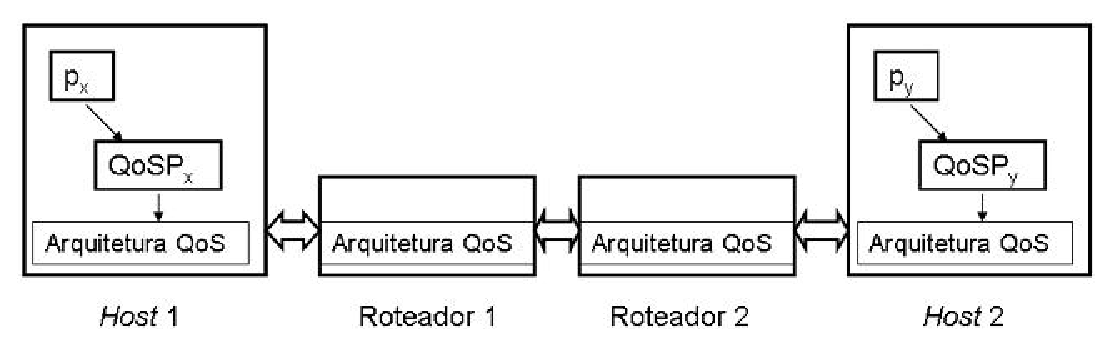
\includegraphics[width=0.3\textwidth]{qosp}
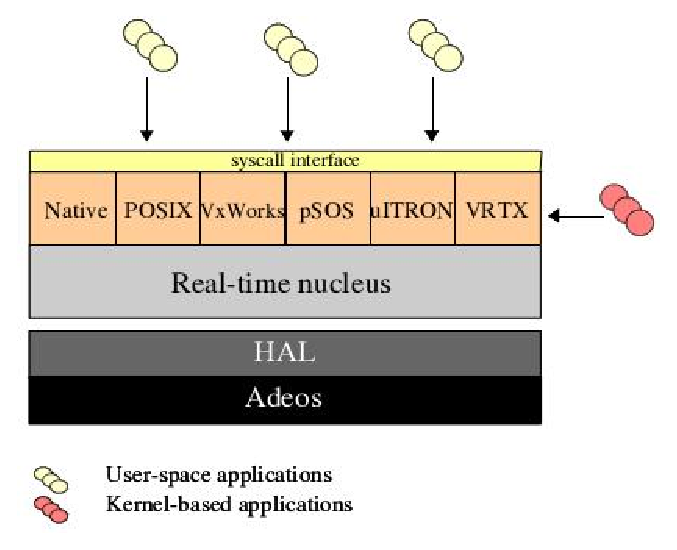
\includegraphics[scale=0.7]{xenomai_skins}
\caption{Skins para o Xenomai \cite{XENO_API06}}
\label{fig:xenomai_skins}
\end{figure}	
	
	O Xenomai utiliza como \textit{micro-kernel} o ADEOS \cite{ADEOS01}, uma camada de abstração do hardware que permite que vários sistemas operacionais compartilhem os recursos de hardware (Figura \ref{fig:xenomai_skins}). O ADEOS trabalha com o conceito de domínios, que são as entidades que coexistem na máquina, onde cada domínio não tem o conhecimento do outro mas todos se comunicam com o ADEOS \cite{ADEOS01}.

	As aplicações de tempo real que são desenvolvidas desde o início tendo como base o Xenomai, geralmente utilizam a API nativa \cite{XENO_API06} do Xenomai. Esta oferece vários serviços disponibilizados comumente nos RTOS \cite{VERGO01} \cite{KALINSKY03}. Os serviços são divididos em seis grandes categorias, sendo que as principais são: gerenciamento de tarefas, serviços de tempo, suporte à sincronização, além de comunicação e transferência de mensagens. Estes serviços podem ser chamados tanto no contexto do espaço do kernel como no contexto do espaço de usuário, permitindo que as aplicações possam executar nos dois contextos.
	
	O Xenomai permite que as tarefas de tempo real executem tanto no domínio do Xenomai (modo primário) como no domínio do Linux (modo secundário), de forma totalmente transparente para os desenvolvedores. Quando uma tarefa executando no domínio do Xenomai faz uma chamada de sistema ao Linux, esta migra para o domínio do Linux, passando a ser gerenciado por este. Quando a execução da chamada de sistema é finalizada, a tarefa volta para o domínio do Xenomai. Para que a previsibilidade possa continuar a ser provida mesmo quando uma tarefa está sob gerência do kernel do Linux, o Xenomai disponibiliza o escudo de interrupção (\textit{Interrupt shield}) \cite{XENO_API06}.
	
	Para que um sistema distribuído possa ter suas restrições de tempo atendidas, além de um kernel de tempo real, é necessário que o sistema de comunicação na rede também forneça garantias temporais. O projeto RTnet, descrito a seguir, visa atender tais requisitos.
	
\section{RTnet}

	O RTnet é um \textit{framework} para comunicação de tempo real rígido sobre Ethernet e outros meios de comunicação \cite{KWZB05}. Enquanto o Xenomai (apresentado anteriormente) se preocupa basicamente com o escalonamento das tarefas de tempo real (está relacionado com o processamento das mensagens), o RTnet foca a transferência das mensagens sobre uma rede Ethernet com restrições rígidas de tempo. Neste caso, podemos observar que o Xenomai e o RTnet se complementam na função de fornecer uma solução para a comunicação em rede que atenda às restrições rígidas de tempo.
	
	Basicamente o RTnet consiste em uma pilha de protocolos de rede capaz de prover comunicação de tempo real sobre Ethernet. Para garantir as restrições rígidas de tempo, o RTnet implementa os protocolos UDP/IP, ICMP e ARP retirando todas as possíveis causas de indeterminismo \cite{KWZB05}.
	
	Além da implementação dos protocolos de forma determinística, o RTnet provê um controle de acesso ao meio determinístico através de sua camada de acesso ao meio denominada RTmac. Com o RTmac, as aplicações de tempo real conseguem obter QoS a um custo baixo, visto que não dependem que um \textit{hardware} implemente a solução de QoS \cite{KWZB05}. Por padrão, a disciplina de acesso ao meio utilizada pelo RTnet para se comunicar na rede Ethernet é o TDMA (\textit{Time Division Multiple Access}). Esta disciplina segue a abordagem mestre-escravo, onde o nó mestre no segmento Ethernet é responsável por sincronizar os relógios dos nós escravos e por definir o momento em que estes podem enviar seus pacotes.